%Resultados

\section{Resultados}\label{sec:resultados}

\subsection{Parte 1. Aplicaciones De Las Topologías Clásicas}\label{subsec:parte1}

    Se tomará en cuenta la incertidumbre de cada uno de los equipos e instrumentos usados en la practica, la documentación de cada equipo se encuentra en los anexos, capitulo \ref{sec:anexos}.

    Las incertidumbres fueron calculadas bajo las ecuaciones que se encuentran en la sección \ref{sec:apendice}, las ecuaciones \ref{eqn:delta_ganancia} y \ref{eqn:delta_corriente}.


    \begin{table}[H]
      \centering
      \begin{tabular}{|c|c|c|cc|c|c|}
        \hline
        \textbf{Topología}                    & \textbf{$V_{cc} [V_{DC}]$}  & \textbf{$V_{EE} [V_{DC}]$}   & \multicolumn{2}{c|}{\textbf{$V_{in}[V_p]$}}                & \textbf{$V_{out} [V_p]$}          & \textbf{$A_v [V/V]$}             \\ \hline
        \textbf{Inversor}                     & $10 \pm 1$                  & $-10 \pm 1$                  & \multicolumn{2}{c|}{$2 \pm 0.2$}                           & $3.8 \pm 0.2$                     & $1.9 \pm 0.39$                   \\ \hline
        \textbf{No inversor}                  & $10 \pm 1$                  & $-10 \pm 1$                  & \multicolumn{2}{c|}{$2 \pm 0.2$}                           & $4\pm 0.2$                        & $2 \pm 0.41$                     \\ \hline
        \multirow{2}{*}{\textbf{Restador}}    & \multirow{2}{*}{$10 \pm 1$} & \multirow{2}{*}{$-10 \pm 1$} & \multicolumn{1}{c|}{$V_1 (V^-)$}        & $V_2 (V^+)$      & \multirow{2}{*}{$1900 \pm 100 m$} & \multirow{2}{*}{$1.63 \pm 0.17$} \\ \cline{4-5}
                                              &                             &                              & \multicolumn{1}{c|}{$ 1800 \pm 100 m $} & $ 640 \pm 40 m $ &                                   &                                  \\ \hline
        \textbf{Integrador Boo} & $10 \pm 1$                  & $-10 \pm 1$                  & \multicolumn{2}{c|}{$ 2.6 \pm 0.2 $}                       & $ 4.8 \pm 0.4 $                   & -                                \\ \hline
      \end{tabular}
      \caption{Mediciones Experimentales de las Primeras Topologías}
      \label{tab:resultados1}
  \end{table}

    \begin{table}[H]
      \centering
      \begin{tabular}{|c|c|c|c|c|}
        \hline
        \textbf{Topología} & $\mathbf{V_{in} [V_{DC}]}$ & $\mathbf{V_{out} [V_{DC}]}$ & $\mathbf{R_L [k \ohm]}$ & $\mathbf{I_o [m A]}$ \\
        \hline
        \multirow{4}{5cm}{\centering \textbf{Fuente de Corriente}} & $4.8 \pm 0.4$ & $320 \pm 20 m$ & $1 \pm 5\%$ & $0.17 \pm 0.026$ \\
        & $4.8 \pm 0.4$ & $520 \pm 40m $ & $3 \pm 5\%$ & $0.32 \pm 0.015$ \\
        & $4.8 \pm 0.4$ & $600 \pm 40m $ & $4 \pm 5\%$ & $0.15 \pm 0.012 $ \\
        & $4.8 \pm 0.4$ & $ 720 \pm 40m $ & $10 \pm 5\%$ & $0.072 \pm 0.005$ \\
        \hline
      \end{tabular}
      \caption{Medición Experimental del Convertidor de Tensión a Corriente, con Distintas Cargas.}
      \label{tab:resultado12}
    \end{table}


    \begin{table}[H]
      \centering
      \begin{tabular}{|c| c| c|}
        \hline
          \textbf{Topología} & $E_{r_{A_v}} [\%]$ & $E_{r_{I}} [\%]$ \\\hline
        Inversor  & $5$ & - \\\hline
        No inversor &  $0$ & - \\\hline
        Restador  &  $18.5$ & - \\\hline
        Fuente de Corriente  &  - & $64.4$ \\\hline
      \end{tabular}
      \caption{Error Porcentual de las Mediciones Experimentales con respecto a las teóricas de las Primeras Topologías}
      \label{tab:desviacion_resultados1}
    \end{table}
    \subsubsection{Inversor}
        \begin{figure}[H]
            \centering
            \renewcommand{\figurename}{Imagen}
            \setcounter{figure}{4}
            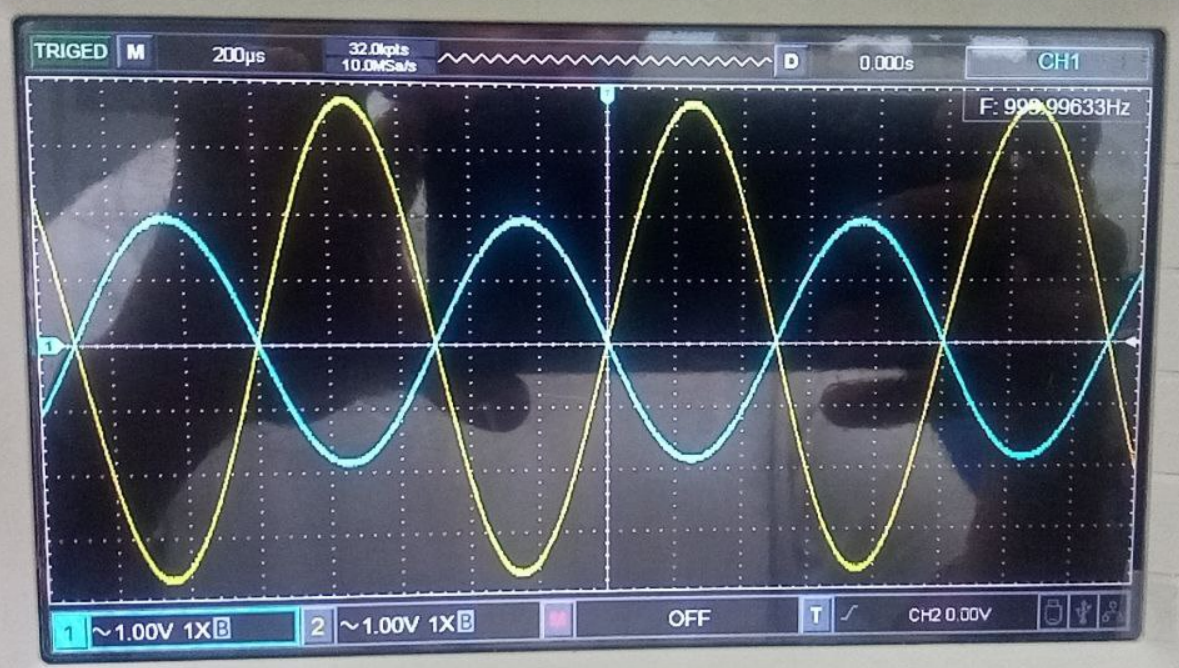
\includegraphics[width=15cm]{Imagenes/exp_inversor.png}
            \caption{Señal de Entrada (Azul) y Salida (Amarilla) del Inversor}
            \label{fig:exp_inversor}
        \end{figure}
    
        \begin{table}[H]
            \centering
            \begin{tabular}{|c|c|c|c|}
                \hline
                \textbf{time/div} $[s]$ & \textbf{Channel} & \textbf{voltios/div $[\volt]$} & \textbf{Acoplamiento} \\ \hline
                $200 \, \mu$ & 1 (Azul) &   $1 $ & AC \\ \hline
                $200 \, \mu$ & 2 (Amarillo)  &   $1 $ & AC \\ \hline  
            \end{tabular}
            \caption{Escalas Usada en el Osciloscopio Digital UNI-T UTD2102CEX+}
            \label{tab:escala_inversor}
        \end{table}

    \subsubsection{No inversor}

        \begin{figure}[H]
            \centering
            \renewcommand{\figurename}{Imagen}
            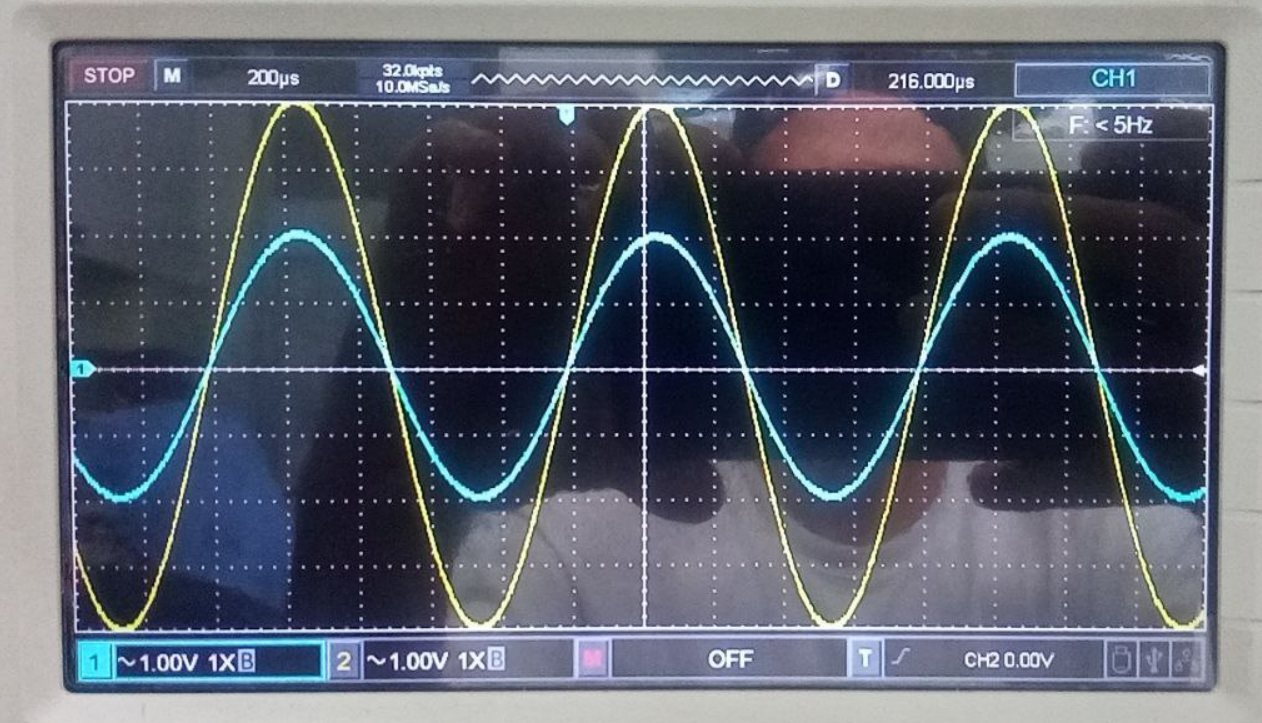
\includegraphics[width=15cm]{Imagenes/exp_noinversor.png}
            \caption{Señal de Entrada (Azul) y Salida (Amarilla) del No Inversor}
            \label{fig:exp_noinversor}
        \end{figure}
    
        \begin{table}[H]
            \centering
            \begin{tabular}{|c|c|c|c|}
                \hline
                \textbf{time/div} $[s]$ & \textbf{Channel} & \textbf{voltios/div $[\volt]$} & \textbf{Acoplamiento} \\ \hline
                $200 \, \mu$ & 1 (Azul) &   $1 $ & AC \\ \hline
                $200 \, \mu$ & 2 (Amarillo)  &   $1 $ & AC \\ \hline  
            \end{tabular}
            \caption{Escalas Usada en el Osciloscopio Digital UNI-T UTD2102CEX+}
            \label{tab:escala_noinversor}
        \end{table}

    \subsubsection{Restador}
        
        
        \begin{figure}[H]
            \centering
            \renewcommand{\figurename}{Imagen}
            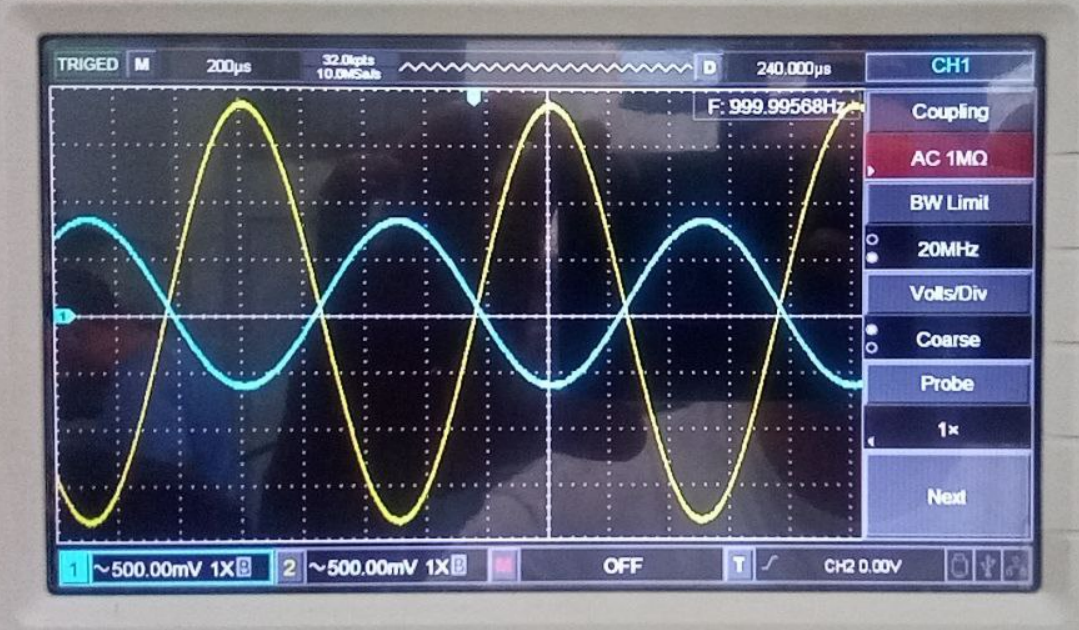
\includegraphics[width=15cm]{Imagenes/exp_restador.png}
            \caption{Señal de Entrada (Azul) y Salida (Amarillo) del Restador}
            \label{fig:exp_restador}
        \end{figure}
    
        \begin{table}[H]
            \centering
            \begin{tabular}{|c|c|c|c|}
                \hline
                \textbf{time/div} $[s]$ & \textbf{Channel} & \textbf{voltios/div $[\volt]$} & \textbf{Acoplamiento} \\ \hline
                $200 \, \mu$ & 1 (Azul) &  $500 \, m $ & AC \\ \hline
                $200 \, \mu$ & 2 (Amarillo)  &   $500 \, m $ & AC \\ \hline  
            \end{tabular}
            \caption{Escalas Usada en el Osciloscopio Digital UNI-T UTD2102CEX+}
            \label{tab:escala_restador}
        \end{table}

    \subsubsection{Integrador No Inversor (Integrador de Boo)}

        \begin{figure}[H]
            \centering
            \renewcommand{\figurename}{Imagen}
            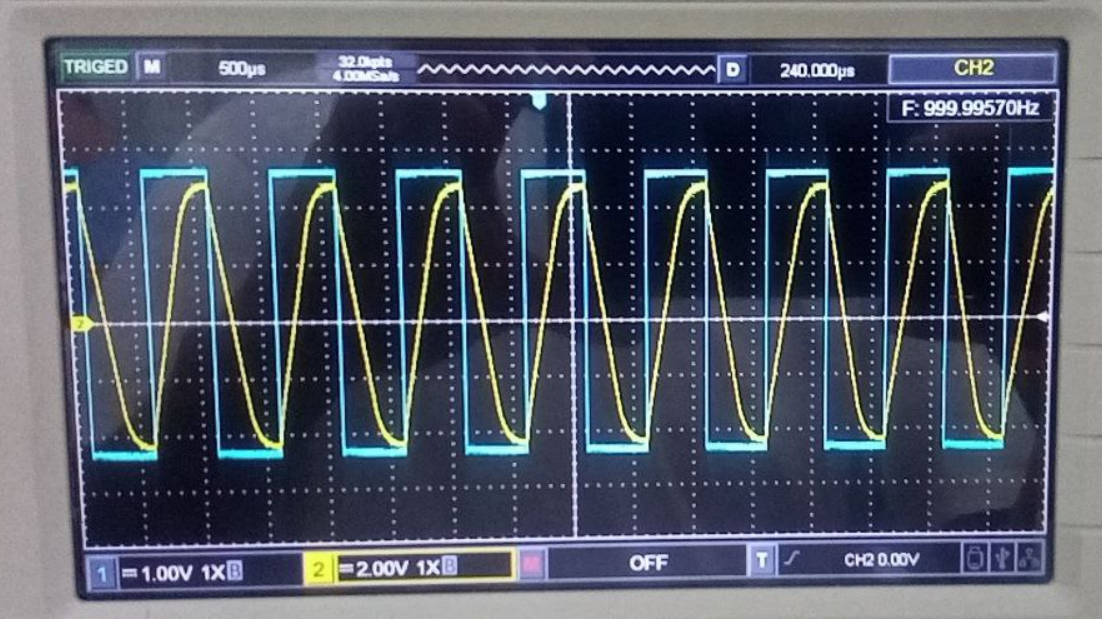
\includegraphics[width=15cm]{Imagenes/exp_integrador_boo.png}
            \caption{Señal de Entrada (Azul) y Salida (Amarilla) del Integrador Boo}
            \label{fig:exp_integrador_boo}
        \end{figure}
    
        \begin{table}[H]
            \centering
            \begin{tabular}{|c|c|c|c|}
                \hline
                \textbf{time/div} $[s]$ & \textbf{Channel} & \textbf{voltios/div $[\volt]$} & \textbf{Acoplamiento} \\ \hline
                $500 \, \mu$ & 1 (Azul) &  $1 $ & AC \\ \hline
                $500 \, \mu$ & 2 (Amarillo)  &   $2 $ & AC \\ \hline  
            \end{tabular}
            \caption{Escalas Usada en el Osciloscopio Digital UNI-T UTD2102CEX+}
            \label{tab:escala_exp_integrador_boo}
        \end{table}

        
\subsection{Parte 2. Amplificador Operacional Real}\label{subsec:parte2}

    En este apartado nos enfocaremos en los resultados experimentales, donde se calcularan las incertidumbres bajo las ecuaciones \ref{eqn:delta_tension_offset}, \ref{eqn:delta_corriente_offset}, \ref{eqn:delta_corriente_polarizacion}\ref{eqn:delta_corriente}, \ref{eqn:delta_gbwp} y \ref{eqn:delta_slewrate}, que se hallan en la sección \ref{sec:apendice} y algunas mediciones indirectas calculadas en el pre-laboratorio, que se hallan en la sección \ref{sec:metodologia}, siendo las ecuaciones \ref{eqn:vos}, \ref{eqn:ib1}, \ref{eqn:ib2}, \ref{eqn:ios} y \ref{eqn:sr}.

    Recordando que JP1 es la entrada inversora, por consiguiente, JP2 es la no inversora.

    Se usaron algunas resistencias de distintos valores, debido a no encontrar las pedidas, con una diferencia del 8.3\% a 10\% con una tolerancia de igual manera de 5\% en la siguiente tabla se indican.

    \begin{table}[H]
        \centering
        \begin{tabular}{|c|c|}
        \hline
           \textbf{Resistencias indicadas} $[\ohm]$  & \textbf{Resistencias usadas} $[\ohm]$\\\hline
            $R_3=R_4=22 \,M  $ & $R_3=R_4=24 \,M \pm 5\%$ \\\hline
            $R_8=910$ & $R_8=820 \pm 5\%$ \\\hline
        \end{tabular}
        \caption{Resistencias Reemplazadas}
        \label{tab:resistencias_reemplazadas}
    \end{table}
    
    \subsubsection{Tensión Offset}

        \begin{table}[H]
          \centering
          \begin{tabular}{|c|c|c|c|c|}
            \hline
            \textbf{Configuración} & $\mathbf{V_{CC} [V_{DC}]}$ & $\mathbf{V_{EE} [V_{DC}]}$ & $\mathbf{V_{o} [V_{DC}]}$ & $\mathbf{V_{os} [mV_{DC}]}$ \\
            \hline
            JP1 y JP2 (corto) & $10 \pm 0.1$ & $-10 \pm 0.1$ & $-2 \pm 0.2$ & $-1.998 \pm 0.245$ \\
            \hline
          \end{tabular}
          \caption{Medición experimental de la Tensión offset de la figura \ref{fig:amp_op_real}}
          \label{tab:tension_offset}
        \end{table}

    \subsubsection{Corriente de Polarización}

        \begin{enumerate}
            \item \textbf{Corriente de polarización 1}

                \begin{table}[H]
                  \centering
                  \begin{tabular}{|c|c|c|c|c|}
                    \hline
                    \textbf{Configuración} & $\mathbf{V_{CC} [V_{DC}]}$ & $\mathbf{V_{EE} [V_{DC}]}$ & $\mathbf{V_{o} [V_{DC}]}$ & $\mathbf{I_{B_1} [pA]}$ \\
                    \hline
                    JP1 (abierto) y JP2 (corto) & $10 \pm 1$ & $-10 \pm 1$ & $-2.6 \pm 0.2$ & $27.245 \pm 16.67$ \\
                    \hline
                  \end{tabular}
                  \caption{Medición experimental de la corriente de polarización de la entrada inversora de la figura \ref{fig:amp_op_real}}
                  \label{tab:corriente_polarizacion1}
                \end{table}

            \item \textbf{Corriente de polarización 2}

                \begin{table}[H]
                  \centering
                  \begin{tabular}{|c|c|c|c|c|}
                    \hline
                    \textbf{Configuración} & $\mathbf{V_{CC} [V_{DC}]}$ & $\mathbf{V_{EE} [V_{DC}]}$ & $\mathbf{V_{o} [V_{DC}]}$ & $\mathbf{I_{B_2} [pA]}$ \\
                    \hline
                    JP1 (corto) y JP2 (abierto) & $10 \pm 0.1$ & $-10 \pm 1$ & $10 \pm 1$ & $544.909 \pm 20.81$ \\
                    \hline
                  \end{tabular}
                  \caption{Medición experimental de la corriente de polarización de la entrada no inversora de la figura \ref{fig:amp_op_real}}
                  \label{tab:corriente_polarizacion2}
                \end{table}
        \end{enumerate}

    \subsubsection{Corriente Offset}

        \begin{table}[H]
          \centering
          \begin{tabular}{|c|}
            \hline
            $\mathbf{I_{os} [pA]}$ \\
            \hline
            $517.664 \pm 26.66$ \\
            \hline
          \end{tabular}
          \caption{Medición indirecta de la corriente de offset, mediante los valores de las tablas \ref{tab:corriente_polarizacion1} y \ref{tab:corriente_polarizacion2}.}
          \label{tab:corriente_offset}
        \end{table} 

    \subsubsection{Producto del Ancho de Banda por la Ganancia (GBWP)}   

        El voltaje de Salida es el voltaje medido justo en su frecuencia de corte, debido que se desea observar su GBWP en las distintas configuraciones.

        \begin{table}[H]
          \centering
          \begin{tabular}{|c|c|c|c|c|}
            \hline
            \textbf{Configuración} & $\mathbf{V_{CC} [V_p]}$ & $\mathbf{V_{EE} [V_p]}$ & $\mathbf{V_{in} [V_p]}$ & $\mathbf{V_{out} [V_p]}$ \\
            \hline
            JP3 y JP4 (abiertos) & $10 \pm 0.1$ & $-10 \pm 0.1$ & $1 \pm 0.1$ & $6 \pm 1$  \\
            \hline
            JP3 (abierto); JP4(corto) & $10 \pm 0.1$ & $-10 \pm 0.1$ & $1 \pm 0.1$  & $6 \, \pm 1$ \\
            \hline
            JP3 y JP4 (corto) Buffer & $10 \pm 0.1$ & $-10 \pm 0.1$ & $1 \pm 0.1$  & $1 \pm 0.1 $ \\
            \hline
          \end{tabular}
        \end{table}
        \begin{table}[H]
          \centering
          \begin{tabular}{|c|c|c|}
            \hline
            \textbf{Configuración} & \textbf{G} $\mathbf{[V/V]}$ & \textbf{F} $\mathbf{[Hz]}$ \\
            \hline
            JP3 y JP4 (abiertos) & $6 \pm 1.166$ & $25 \pm 6.25 \, k $ \\
            \hline
            JP3 (abierto); JP4(corto) & $6 \pm 1.116$ & $25 \pm 6.25 \, k$ \\
            \hline
            JP3 y JP4 (corto) Buffer & $1 \pm 0.141$ & Un valor muy grande se distorsiona \\
            \hline
          \end{tabular}
          \caption{Mediciones experimentales del GBWP de la figura \ref{fig:GBWP}}
          \label{tab:gbwp}
        \end{table}

         \begin{table}[H]
          \centering
          \begin{tabular}{|c|c|}
            \hline
            \textbf{Configuración} & \textbf{GBWP} $[(V/V)Hz$ \\
            \hline
            JP3 y JP4 (abiertos) & $150\pm 15.31 \, k$ \\
            \hline
            JP3 (abierto); JP4(corto) & $150 \pm  15.31 \, k$ \\
            \hline
            JP3 y JP4 (corto) Buffer & Muy grande \\
            \hline
          \end{tabular}
          \caption{Calculo del GBWP de la figura \ref{fig:GBWP}}
          \label{tab:calculo_gbwp}
        \end{table}
        Reflejando la ganancia y la frecuencia en un plano cartesiano de Ganancia vs Frecuencia, se puede visualizar mejor los puntos de las mediciones experimentales en la gráfica \ref{fig:puntos_gbwp}.

        \begin{figure}[H]
            \centering
            \renewcommand{\figurename}{Gráfica}
            \setcounter{figure}{36}
            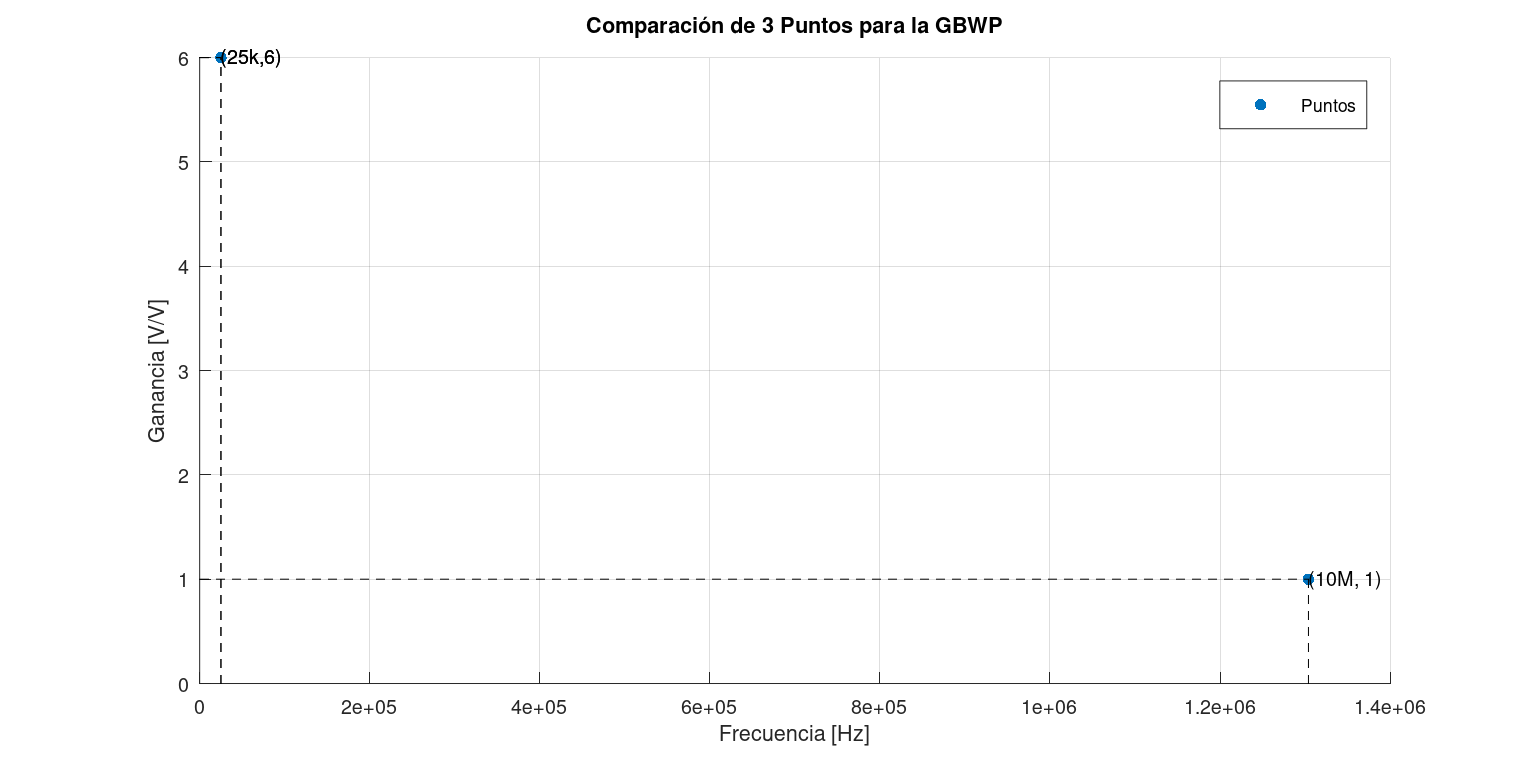
\includegraphics[width=15cm]{Imagenes/puntos_gbwp.png}
            \caption{Puntos reflejados de la Ganancia Vs Frecuencia, cumpliendo el Producto  del Ancho de Banda por la Ganancia (GBWP)}
            \label{fig:puntos_gbwp}
        \end{figure}

    \subsubsection{Slew Rate(SR) o Tasa de Variación}

        Acá haremos uso de la mediciones indirectas de la ecuación \ref{eqn:sr}, bajo las mediciones realizadas con el osciloscopio digital.
        
        \begin{figure}[H]
            \centering
            \renewcommand{\figurename}{Imagen}
            \setcounter{figure}{11}
            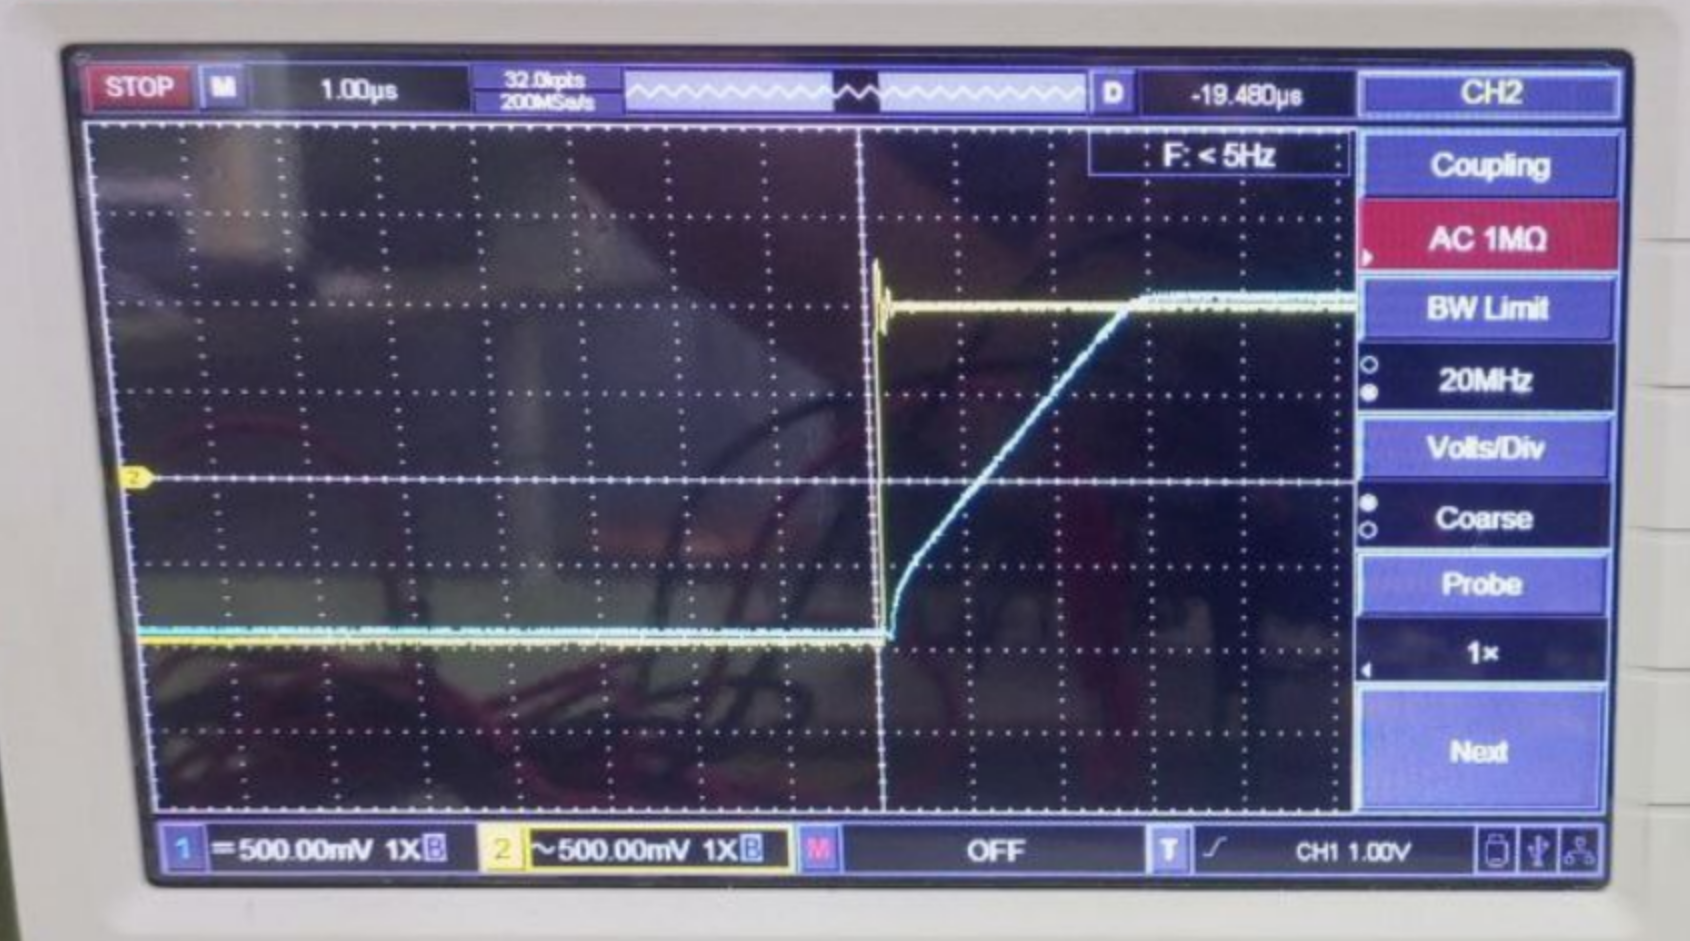
\includegraphics[width=15cm]{Imagenes/exp_sr.png}
            \caption{Señal de Salida (Azul) y Entrada (Amarilla) del Buffer, donde se puede observar la tasa de variación en su señal de salida de la figura \ref{fig:buffer}}
            \label{fig:exp_sr}
        \end{figure}

        \begin{table}[H]
            \centering
            \begin{tabular}{|c|c|c|c|}
                \hline
                \textbf{time/div} $[s]$ & \textbf{Channel} & \textbf{voltios/div $[\volt]$} & \textbf{Acoplamiento} \\ \hline
                $1 \, \mu$ & 1 (Azul) &  $500 \, m $ & AC \\ \hline
                $1 \, \mu$ & 2 (Amarillo)  &   $500 \, m $ & AC \\ \hline  
            \end{tabular}
            \caption{Escalas Usada en el Osciloscopio Digital UNI-T UTD2102CEX+}
            \label{tab:escala_exp_sr}
        \end{table}

        \begin{table}[H]
          \centering
          \begin{tabular}{|c|c|c|c|c|c|c|c|c|}
            \hline
            $\mathbf{V_{CC} [V_p]}$ & $\mathbf{V_{EE} [V_p]}$ & $\mathbf{V_{in} [mV_p]}$ & $\mathbf{t_1 [\mu s]}$ & $\mathbf{t_2 [\mu s]}$ & $\mathbf{V_1 [mV]}$ & $\mathbf{V_2 [mV]}$ & $\mathbf{SR [V/\mu s]}$ \\
            \hline
            $10 \pm 0.1$ & $-10 \pm 0.1$ & $1000 \pm 100$ & $0.3 \pm 0.2$ & $2.7 \pm 0.2$ & $-500 \pm 100$ & $700 \pm 100$ & $0.5 \pm 0.05$ \\
            \hline
          \end{tabular}
          \caption{Mediciones del Slew Rate de la figura \ref{fig:buffer}}
          \label{tab:exp_sr}
        \end{table}

    \subsubsection{Corriente de Cortocircuito}

        \begin{table}[H]
          \centering
          \begin{tabular}{|c|c|c|c|c|c|}
            \hline
            $\mathbf{V_{CC} [V_p]}$ & $\mathbf{V_{EE} [V_p]}$ & $\mathbf{V_{in} [V_p]}$ & $\mathbf{V_o [V_p]}$ & $\mathbf{R_v [\ohm]}$ & $\mathbf{I_{CC} [mA]}$ \\
            \hline
            $10 \pm 0.1$ & $-10 \pm 0.1$ & $5 \pm 1$ & $0.1 \pm 0.02$ & $3.9 \pm 5\%$ & $25.64 \pm 5.29$ \\
            \hline
          \end{tabular}
          \caption{Mediciones Experimentales de la Corriente de Cortocircuito de la Figura \ref{fig:bufferv}}
          \label{tab:corriente_cc}
        \end{table}

    \subsubsection{Límites Máximos de Excursión}    

        \begin{figure}[H]
            \centering
            \renewcommand{\figurename}{Imagen}
            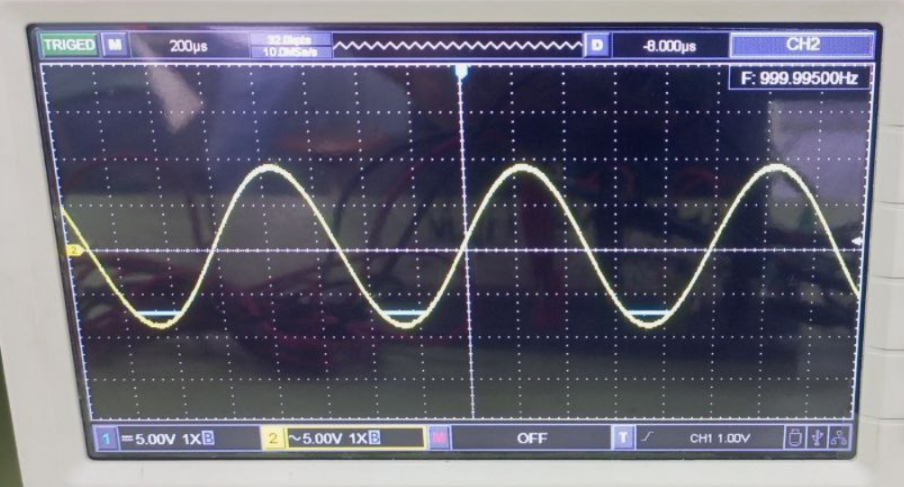
\includegraphics[width=15cm]{Imagenes/exp_buffer_limites.png}
            \caption{Señal de Salida (Azul) y Entrada (Amarilla) del Buffer, donde se puede observar los limites máximos de excursión en su señal de salida de la figura \ref{fig:buffer}}
            \label{fig:exp_buffer_limites}
        \end{figure}

        \begin{table}[H]
            \centering
            \begin{tabular}{|c|c|c|c|}
                \hline
                \textbf{time/div} $[s]$ & \textbf{Channel} & \textbf{voltios/div $[\volt]$} & \textbf{Acoplamiento} \\ \hline
                $200 \, \mu$ & 1 (Azul) &  $5 $ & AC \\ \hline
                $200 \, \mu$ & 2 (Amarillo)  &   $5 $ & AC \\ \hline  
            \end{tabular}
            \caption{Escalas Usada en el Osciloscopio Digital UNI-T UTD2102CEX+}
            \label{tab:escala_exp_buffer_limites}
        \end{table}

        \begin{table}[H]
          \centering
          \begin{tabular}{|c|c|}
            \hline
            \textbf{Limites máximos} & $\mathbf{V_o [V_p]}$ \\
            \hline
            Superior & $9 \pm 1$ \\
            \hline
            Inferior & $7 \pm 1$ \\
            \hline
          \end{tabular}
          \caption{Mediciones Experimentales de los Límites Máximos de Excursión de la Figura \ref{fig:buffer}}
          \label{tab:exp_buffer_limites}
        \end{table}

    
\subsection{Parte 3. Filtros Activos}\label{subsec:parte3}

      En este apartado, se calcularan las incertidumbres de ganancia y frecuencia, siendo las ecuaciones \ref{eqn:delta_frecuencia} y \ref{eqn:delta_ganancia}, que se hallan en la sección \ref{sec:apendice}. Las figuras que se le realizaron las mediciones experimentales fueron la \ref{fig:var_estado}, \ref{fig:sallen_key} y \ref{fig:retro_multiples}. 
      
      A continuación se procede a indicar los resultados.

      \subsubsection{Filtro de Variables de Estado}

        \begin{itemize}
          \item \textbf{Pasa Bajos}
        
            En este apartado, se diseño el circuito que se pedía solo para la salida del pasa bajo, sin embargo, fueron simuladas las otras salidas y concuerdan con los resultados obtenidos.

            \begin{table}[H]
              \centering
              \begin{tabular}{|c|c|c|c|c|c|c|}
                \hline
                $\mathbf{V_{CC} [V_p]}$ & $\mathbf{V_{EE} [V_p]}$ & $\mathbf{V_{in} [V_p]}$ & $\mathbf{V_{out} [V_p]}$ & \textbf{Ganancia} $\mathbf{[V/V]}$ & \textbf{Frecuencia} $\mathbf{[Hz]}$ \\
                \hline
                $10 \pm 0.1$ & $-10 \pm 0.1$ & $1 \pm 0.1$ & $1.9 \pm 0.1$ & $1.9 \pm 0.21$ & $1 \pm 0.04 k$ \\
                \hline
                $10 \pm 0.1$ & $-10 \pm 0.1$ & $1 \pm 0.1$ & $1.8 \pm 0.1$ & $1.8 \pm 0.21$ & $1.5 \pm 0.045 k$ \\
                \hline
                $10 \pm 0.1$ & $-10 \pm 0.1$ & $1 \pm 0.1$ & $1.7 \pm 0.1 $ & $1.7 \pm 0.20$ & $2 \pm 0.08 k$ \\
                \hline
                $10 \pm 0.1$ & $-10 \pm 0.1$ & $1 \pm 0.1$ & $1.2 \pm 0.1$ & $1.2 \pm 0.16$ & $3.2 \pm 0.205 k$ \\
                \hline
                $10 \pm 0.1$ & $-10 \pm 0.1$ & $1 \pm 0.1$ & $1 \pm 0.1$ & $1 \pm 0.14$ & $3.5 \pm 0.123 k$ \\
                \hline
                $10 \pm 0.1$ & $-10 \pm 0.1$ & $1 \pm 0.1$ & $0.5 \pm 0.1$ & $0.5 \pm 0.11$ & $5.5 \pm 0.303 k$ \\
                \hline
              \end{tabular}
              \caption{Medidas y Cálculos Experimentales de la Ganancia y Frecuencia de la Figura \ref{fig:var_estado}}
              \label{tab:exp_var_estado}
            \end{table}

            \begin{table}[H]
              \centering
              \begin{tabular}{|c|c|c|c|}
                \hline
                $\mathbf{f_{c_{exp}} [Hz]}$ & $\mathbf{f_{c_{teo}} [Hz]}$ & \textbf{Desviación de frecuencia [\%]} \\
                \hline
                $3.5 \pm 0.123  \, k$ & $2.74 \pm 0.55 \, k$ & $21.71$ \\
                \hline
              \end{tabular}
              \caption{Desviación Estándar de la Frecuencia de Corte de la Figura \ref{fig:var_estado}}
              \label{tab:exp_var_estado_frecorte}
            \end{table}

            Haciendo uso de la tabla \ref{tab:exp_var_estado}, tomando los valores que se hallan en las columnas de Ganancia y frecuencia, se puede obtener el Diagrama  Asintótico de Bode en magnitud (respuesta en frecuencia) como se tiene en la gráfica \ref{fig:resp_frec_var_estado} a continuación.

             \begin{figure}[H]
                \centering
                \renewcommand{\figurename}{Gráfica}
                \setcounter{figure}{37}
                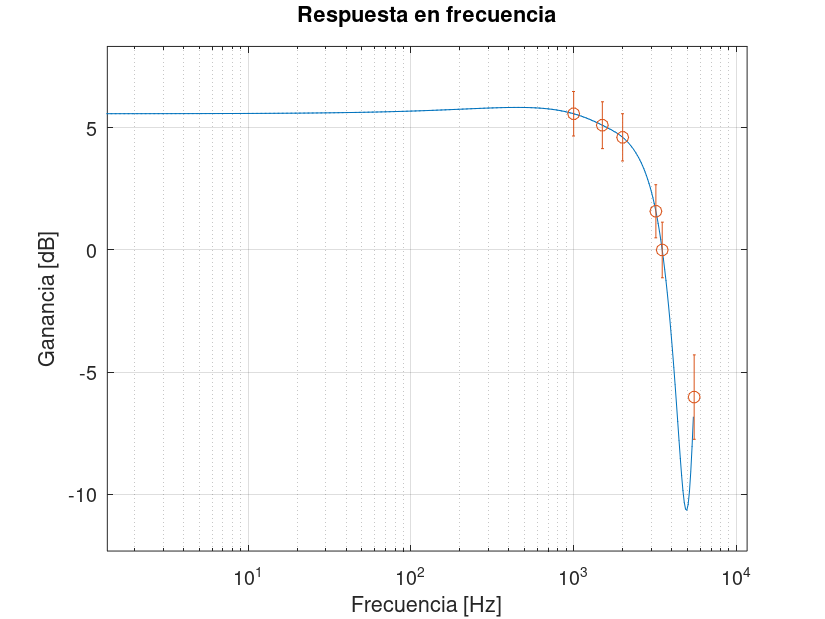
\includegraphics[width=15cm]{Imagenes/resp_frec_var_estado.png}
                \caption{Diagrama  Asintótico de Bode en magnitud (respuesta en frecuencia pasa bajo) de las mediciones experimentales de la tabla \ref{tab:exp_var_estado}}
                \label{fig:resp_frec_var_estado}
            \end{figure}

            El gráfico \ref{fig:resp_frec_var_estado}, fue generado por el lenguaje de programación GNU Octave, el código se encuentra en la sección \ref{sec:anexos}, en la división \ref{subsec:cod_octave}, denominado \textbf{Diagrama asintótico de Bode}, además todas las respuestas en frecuencia se hallarán a través del mismo script.
            \begin{itemize}
                \item \textbf{Armónicos}

                     \begin{figure}[H]
                        \centering
                        \renewcommand{\figurename}{Imagen}
                        \setcounter{figure}{13}
                        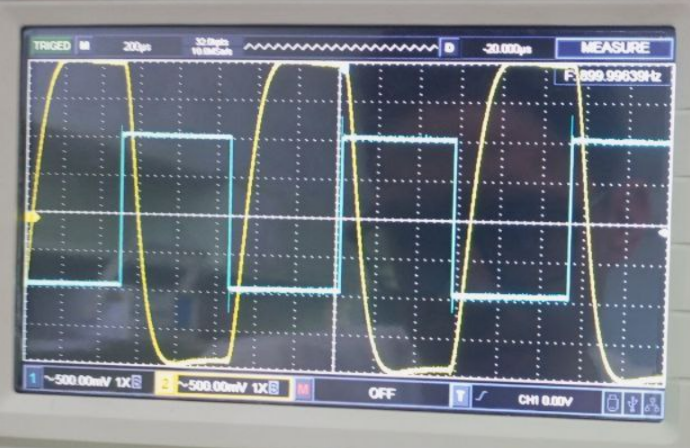
\includegraphics[width=15cm]{Imagenes/armonico_var_estado.png}
                        \caption{Señal de Entrada (Azul) y Salida (Amarilla), donde se puede observar los cambios en la señal de salida con su tercer armónico coincidiendo con la frecuencia de corte teórico de la tabla \ref{tab:exp_var_estado_frecorte}}
                        \label{fig:armonico_var_estado}
                    \end{figure}
            
                    \begin{table}[H]
                        \centering
                        \begin{tabular}{|c|c|c|c|}
                            \hline
                            \textbf{time/div} $[s]$ & \textbf{Channel} & \textbf{voltios/div $[\volt]$} & \textbf{Acoplamiento} \\ \hline
                            $200 \, \mu$ & 1 (Azul) &  $500 \, m $ & AC \\ \hline
                            $200 \, \mu$ & 2 (Amarillo)  &   $500 \, m $ & AC \\ \hline  
                        \end{tabular}
                        \caption{Escalas Usada en el Osciloscopio Digital UNI-T UTD2102CEX+}
                        \label{tab:escala_exp_var_estado_armonico}
                    \end{table}
            \end{itemize}

            \item \textbf{Pasa Banda}
            
            \begin{table}[H]
              \centering
              \begin{tabular}{|c|c|c|c|c|c|c|}
                \hline
                $\mathbf{V_{CC} [V_p]}$ & $\mathbf{V_{EE} [V_p]}$ & $\mathbf{V_{in} [V_p]}$ & $\mathbf{V_{out} [mV_p]}$ & \textbf{Ganancia} $\mathbf{[V/V]}$ & \textbf{Frecuencia} $\mathbf{[Hz]}$ \\
                \hline
                $10 \pm 0.1$ & $-10 \pm 0.1$ & $1 \pm 0.1$ & $200 \pm 20$ & $0.2 \pm 0.028$ & $700 \pm 49 $ \\
                \hline
                $10 \pm 0.1$ & $-10 \pm 0.1$ & $1 \pm 0.1$ & $360 \pm 20$ & $0.32 \pm 0.041$ & $1.3 \pm 0.068 k$ \\
                \hline
                $10 \pm 0.1$ & $-10 \pm 0.1$ & $1 \pm 0.1$ & $520 \pm 40 $ & $0.52 \pm 0.066$ & $3.5 \pm 0.25 k$ \\
                \hline
                $10 \pm 0.1$ & $-10 \pm 0.1$ & $1 \pm 0.1$ & $360 \pm 20$ & $0.36 \pm 0.041$ & $6.2 \pm 0.38 k$ \\
                \hline
                $10 \pm 0.1$ & $-10 \pm 0.1$ & $1 \pm 0.1$ & $200 \pm 20$ & $0.2 \pm 0.028$ & $12.4 \pm 0.62 k$ \\
                \hline
              \end{tabular}
              \caption{Medidas y Cálculos Experimentales de la Ganancia y Frecuencia de la Figura \ref{fig:var_estado}}
              \label{tab:exp_var_estado_pb}
            \end{table}

            \begin{table}[H]
              \centering
              \begin{tabular}{|c|c|}
                \hline
                $\mathbf{f_{c_{exp_L}} [Hz]}$ & $\mathbf{f_{c_{exp_H}} [Hz]}$  \\
                \hline
                $1.3 \pm 0.068 k$ & $6.2 \pm 0.38 k$ \\
                \hline
              \end{tabular}
              \caption{Desviación Estándar de la Frecuencia de Corte de la Figura \ref{fig:var_estado}}
              \label{tab:exp_var_estado_frecorte_pb}
            \end{table}

            Haciendo uso de la tabla \ref{tab:exp_var_estado_pb}, tomando los valores que se hallan en las columnas de Ganancia y frecuencia, se puede obtener el Diagrama  Asintótico de Bode en magnitud (respuesta en frecuencia) como se tiene en la gráfica \ref{fig:resp_frec_var_estado_pb} a continuación.

             \begin{figure}[H]
                \centering
                \renewcommand{\figurename}{Gráfica}
                \setcounter{figure}{38}
                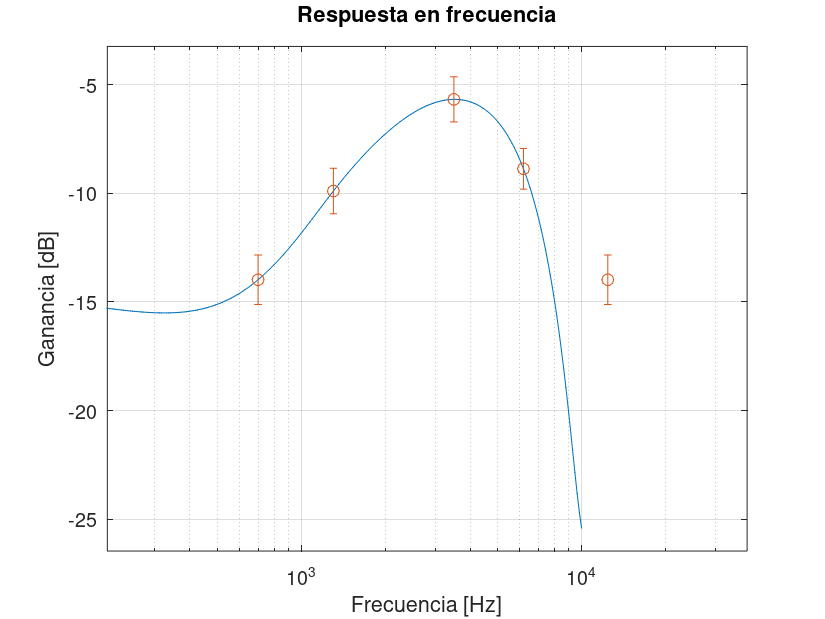
\includegraphics[width=15cm]{Imagenes/resp_frec_var_estado_pb.png}
                \caption{Diagrama  Asintótico de Bode en magnitud (respuesta en frecuencia pasa banda) de las mediciones experimentales de la tabla \ref{tab:exp_var_estado_pb}}
                \label{fig:resp_frec_var_estado_pb}
            \end{figure}

            \item \textbf{Pasa Altos}
            
            
            \begin{table}[H]
              \centering
              \begin{tabular}{|c|c|c|c|c|c|c|}
                \hline
                $\mathbf{V_{CC} [V_p]}$ & $\mathbf{V_{EE} [V_p]}$ & $\mathbf{V_{in} [V_p]}$ & $\mathbf{V_{out} [mV_p]}$ & \textbf{Ganancia} $\mathbf{[V/V]}$ & \textbf{Frecuencia} $\mathbf{[Hz]}$ \\
                \hline
                $10 \pm 0.1$ & $-10 \pm 0.1$ & $1 \pm 0.1$ & $180 \pm 10$ & $0.18 \pm 0.020$ & $2 \pm 0.08 k$ \\
                \hline
                $10 \pm 0.1$ & $-10 \pm 0.1$ & $1 \pm 0.1$ & $300 \pm 20$ & $0.3 \pm 0.036$ & $3 \pm 0.18 k$ \\
                \hline
                $10 \pm 0.1$ & $-10 \pm 0.1$ & $1 \pm 0.1$ & $400 \pm 20 $ & $0.40 \pm 0.045$ & $5 \pm 0.25 k$ \\
                \hline
                $10 \pm 0.1$ & $-10 \pm 0.1$ & $1 \pm 0.1$ & $440 \pm 40$ & $0.44 \pm 0.060$ & $10 \pm 0.40 k$ \\
                \hline
              \end{tabular}
              \caption{Medidas y Cálculos Experimentales de la Ganancia y Frecuencia de la Figura \ref{fig:var_estado}}
              \label{tab:exp_var_estado_pa}
            \end{table}

            
            \begin{table}[H]
              \centering
              \begin{tabular}{|c|}
                \hline
                $\mathbf{f_{c_{exp} [Hz]}}$ \\
                \hline
                $3 \pm 0.068 k$  \\
                \hline
              \end{tabular}
              \caption{Desviación Estándar de la Frecuencia de Corte de la Figura \ref{fig:var_estado}}
              \label{tab:exp_var_estado_frecorte_pa}
            \end{table}

            Haciendo uso de la tabla \ref{tab:exp_var_estado_pa}, tomando los valores que se hallan en las columnas de Ganancia y frecuencia, se puede obtener el Diagrama  Asintótico de Bode en magnitud (respuesta en frecuencia) como se tiene en la gráfica \ref{fig:resp_frec_var_estado_pa} a continuación.

             \begin{figure}[H]
                \centering
                \renewcommand{\figurename}{Gráfica}
                \setcounter{figure}{39}
                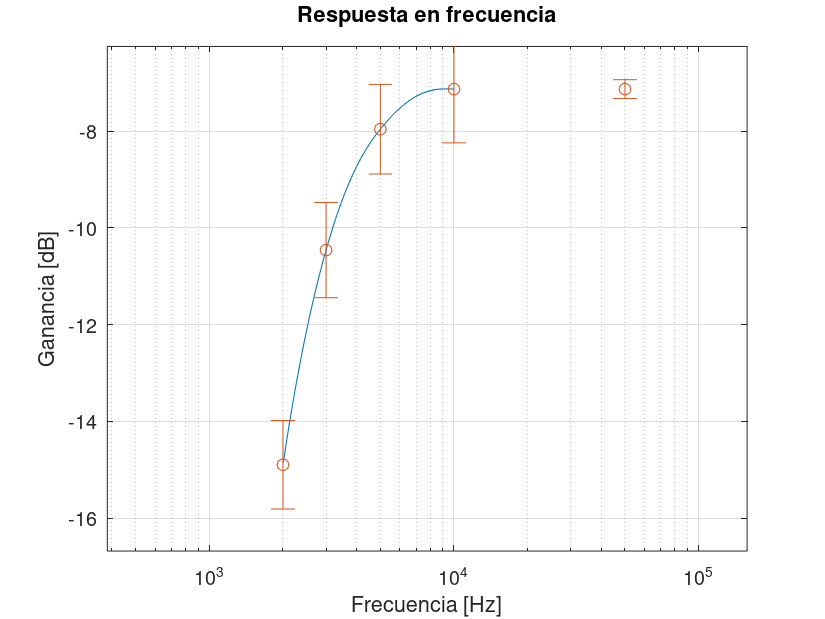
\includegraphics[width=15cm]{Imagenes/resp_frec_var_estado_pa.png}
                \caption{Diagrama  Asintótico de Bode en magnitud (respuesta en frecuencia pasa altos) de las mediciones experimentales de la tabla \ref{tab:exp_var_estado_pa}}
                \label{fig:resp_frec_var_estado_pa}
            \end{figure}

          \end{itemize}

        \subsubsection{Filtro Pasa Bajos con Topología Sallen-Key}

            \begin{table}[H]
              \centering
              \begin{tabular}{|c|c|c|c|c|c|c|}
                \hline
                $\mathbf{V_{CC} [V_p]}$ & $\mathbf{V_{EE} [V_p]}$ & $\mathbf{V_{in} [V_p]}$ & $\mathbf{V_{out} [V_p]}$ & \textbf{Ganancia} $\mathbf{[V/V]}$ & \textbf{Frecuencia} $\mathbf{[Hz]}$ \\
                \hline
                $10 \pm 0.1$ & $-10 \pm 0.1$ & $1 \pm 0.1$ & $2 \pm 0.1$ & $2 \pm 0.22$ & $100 \pm 4 $ \\
                \hline
                $10 \pm 0.1$ & $-10 \pm 0.1$ & $1 \pm 0.1$ & $2.2 \pm 0.2$ & $2.2 \pm 0.29$ & $1 \pm 0.40 k$ \\
                \hline
                $10 \pm 0.1$ & $-10 \pm 0.1$ & $1 \pm 0.1$ & $1.5 \pm 0.1 $ & $1.5 \pm 0.18$ & $5.4 \pm 0.29 k$ \\
                \hline
                $10 \pm 0.1$ & $-10 \pm 0.1$ & $1 \pm 0.1$ & $1 \pm 0.1$ & $1 \pm 0.14$ & $8.1 \pm 0.66 k$ \\
                \hline
                $10 \pm 0.1$ & $-10 \pm 0.1$ & $1 \pm 0.1$ & $ 0.48\pm 0.04$ & $0.48 \pm 0.062$ & $17 \pm 0.58 k$ \\
                \hline
              \end{tabular}
              \caption{Medidas y Cálculos Experimentales de la Ganancia y Frecuencia de la Figura \ref{fig:sallen_key}}
              \label{tab:exp_sallen_key}
            \end{table}

            \begin{table}[H]
              \centering
              \begin{tabular}{|c|c|c|c|}
                \hline
                $\mathbf{f_{c_{exp}} [Hz]}$ & $\mathbf{f_{c_{teo}} [Hz]}$ & \textbf{Desviación de frecuencia [\%]} \\
                \hline
                $5.4 \pm 0.29 \, k$ & $2.74 \pm 0.55 \, k$ & $97.08$ \\
                \hline
              \end{tabular}
              \caption{Desviación Estándar de la Frecuencia de Corte de la Figura \ref{fig:sallen_key}}
              \label{tab:exp_sallen_key_frecorte}
            \end{table}
    
            Haciendo uso de la tabla \ref{tab:exp_sallen_key}, tomando los valores que se hallan en las columnas de Ganancia y frecuencia, se puede obtener el Diagrama  Asintótico de Bode en magnitud (respuesta en frecuencia) como se tiene en la gráfica \ref{fig:resp_frec_sallen_key} a continuación.

            \begin{figure}[H]
                \centering
                \renewcommand{\figurename}{Gráfica}
                \setcounter{figure}{40}
                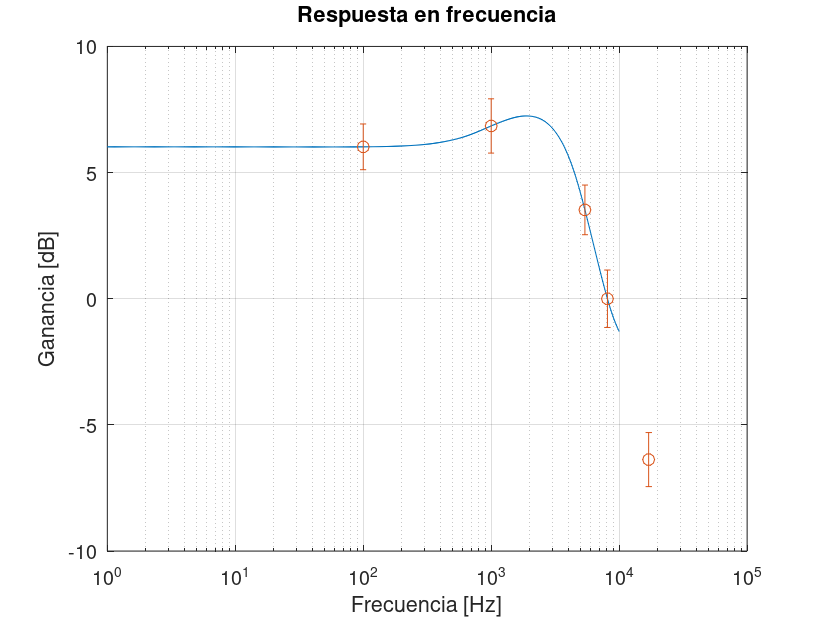
\includegraphics[width=15cm]{Imagenes/resp_frec_sallen_key.png}
                \caption{Diagrama  Asintótico de Bode en magnitud (respuesta en frecuencia) de las mediciones experimentales de la tabla \ref{tab:exp_sallen_key}}
                \label{fig:resp_frec_sallen_key}
            \end{figure}

             \begin{itemize}
                \item \textbf{Armónicos}

                     \begin{figure}[H]
                        \centering
                        \renewcommand{\figurename}{Imagen}
                        \setcounter{figure}{14}
                        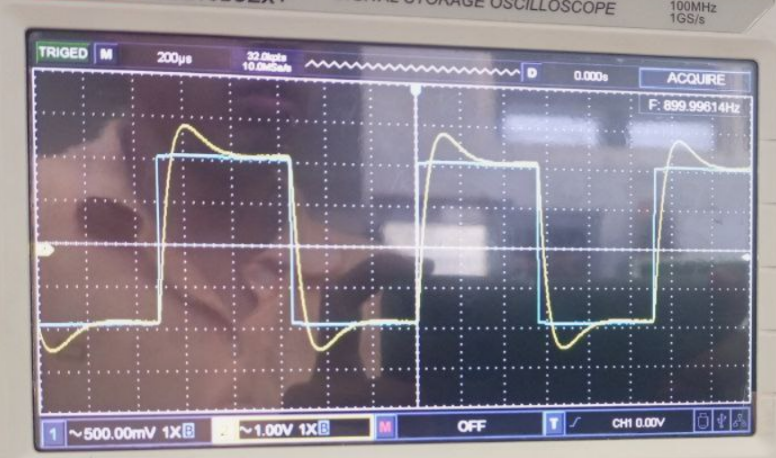
\includegraphics[width=15cm]{Imagenes/armonico_sallen_key.png}
                        \caption{Señal de Entrada (Azul) y Salida (Amarilla), donde se puede observar los cambios en la señal de salida con su tercer armónico coincidiendo con la frecuencia de corte teórico de la tabla \ref{tab:exp_sallen_key_frecorte}}
                        \label{fig:armonico_sallen_key}
                    \end{figure}
            
                    \begin{table}[H]
                        \centering
                        \begin{tabular}{|c|c|c|c|}
                            \hline
                            \textbf{time/div} $[s]$ & \textbf{Channel} & \textbf{voltios/div $[\volt]$} & \textbf{Acoplamiento} \\ \hline
                            $100 \, \mu$ & 1 (Azul) &  $500 \, m $ & AC \\ \hline
                            $100 \, \mu$ & 2 (Amarillo)  &   $500 \, m $ & AC \\ \hline  
                        \end{tabular}
                        \caption{Escalas Usada en el Osciloscopio Digital UNI-T UTD2102CEX+}
                        \label{tab:escala_exp_sallen_key_armonico}
                    \end{table}
            \end{itemize}

        \subsubsection{Filtro Pasa Bajos con Topología de Retroalimentaciones Múltiples}    

            \begin{table}[H]
              \centering
              \begin{tabular}{|c|c|c|c|c|c|}
                \hline
                $\mathbf{V_{CC} [V_p]}$ & $\mathbf{V_{EE} [V_p]}$ & $\mathbf{V_{in} [V_p]}$ & $\mathbf{V_{out} [V_p]}$ & \textbf{Ganancia} $\mathbf{[V/V]}$ & \textbf{Frecuencia} $\mathbf{[Hz]}$ \\
                \hline
                $10 \pm 0.1$ & $-10 \pm 0.1$ & $1 \pm 0.1$ & $1.9 \pm 0.1$ & $1.9 \pm 0.21$ & $100 \pm 40 $ \\
                \hline
                $10 \pm 0.1$ & $-10 \pm 0.1$ & $1 \pm 0.1$ & $1.9 \pm 0.2$ & $1.9 \pm 0.28$ & $1 \pm 0.40 k$ \\
                \hline
                $10 \pm 0.1$ & $-10 \pm 0.1$ & $1 \pm 0.1$ & $1.4 \pm 0.1 $ & $1.4 \pm 0.17$ & $2.8 \pm 0.16 k$ \\
                \hline
                $10 \pm 0.1$ & $-10 \pm 0.1$ & $1 \pm 0.1$ & $0.8 \pm 0.1$ & $0.8 \pm 0.13$ & $4.1 \pm 0.17 k$ \\
                \hline
                $10 \pm 0.1$ & $-10 \pm 0.1$ & $1 \pm 0.1$ & $ 0.6 \pm 0.04$ & $0.6 \pm 0.072$ & $4.9 \pm 0.24 k$ \\
                \hline
              \end{tabular}
              \caption{Medidas y Cálculos Experimentales de la Ganancia y Frecuencia de la Figura \ref{fig:retro_multiples}}
              \label{tab:exp_retro_multiples}
            \end{table}

             \begin{table}[H]
              \centering
              \begin{tabular}{|c|c|c|c|}
                \hline
                $\mathbf{f_{c_{exp}} [Hz]}$ & $\mathbf{f_{c_{teo}} [Hz]}$ & \textbf{Desviación de frecuencia [\%]} \\
                \hline
                $2.8 \pm 0.16 k$ & $2.42 \pm 0.48 \, k$ & $15.70$ \\
                \hline
              \end{tabular}
              \caption{Desviación Estándar de la Frecuencia de Corte de la Figura \ref{fig:retro_multiples}}
              \label{tab:exp_retro_multiples_frecorte}
            \end{table}

             Haciendo uso de la tabla \ref{tab:exp_retro_multiples}, tomando los valores que se hallan en las columnas de Ganancia y frecuencia, se puede obtener el Diagrama  Asintótico de Bode en magnitud (respuesta en frecuencia) como se tiene en la gráfica \ref{fig:resp_frec_retro_multiples} a continuación.

             \begin{figure}[H]
                \centering
                \renewcommand{\figurename}{Gráfica}
                \setcounter{figure}{41}
                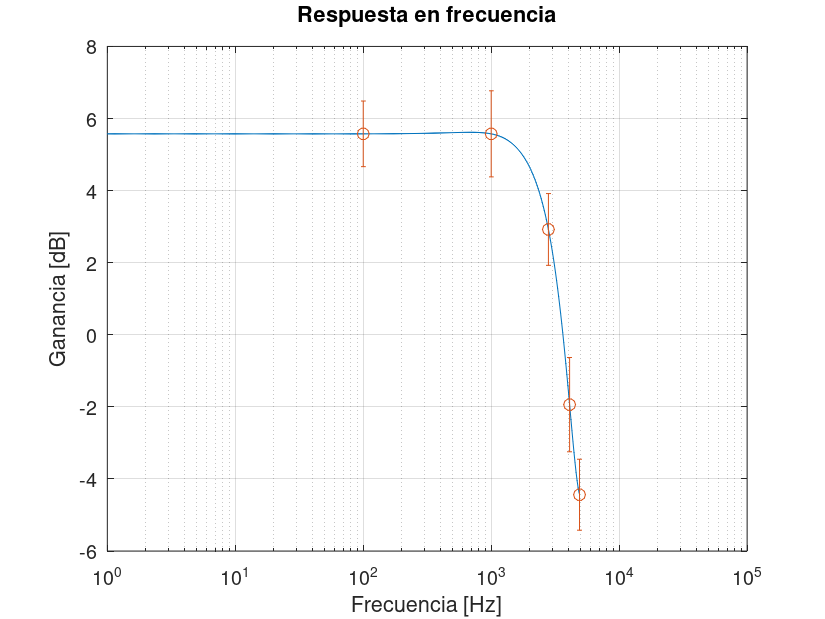
\includegraphics[width=15cm]{Imagenes/resp_frec_retro_multiples.png}
                \caption{Diagrama  Asintótico de Bode en magnitud (respuesta en frecuencia) de las mediciones experimentales de la tabla \ref{tab:exp_retro_multiples}}
                \label{fig:resp_frec_retro_multiples}
            \end{figure}

             \begin{itemize}
                \item \textbf{Armónicos}

                     \begin{figure}[H]
                        \centering
                        \renewcommand{\figurename}{Imagen}
                        \setcounter{figure}{15}
                        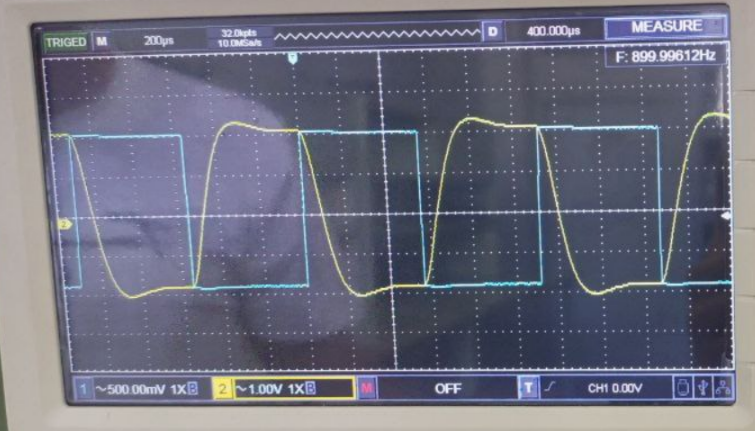
\includegraphics[width=15cm]{Imagenes/armonico_retro_multiples.png}
                        \caption{Señal de Entrada (Azul) y Salida (Amarilla), donde se puede observar los cambios en la señal de salida con su tercer armónico coincidiendo con la frecuencia de corte teórico de la tabla \ref{tab:exp_retro_multiples_frecorte}}
                        \label{fig:armonico_retro_multiples}
                    \end{figure}
            
                    \begin{table}[H]
                        \centering
                        \begin{tabular}{|c|c|c|c|}
                            \hline
                            \textbf{time/div} $[s]$ & \textbf{Channel} & \textbf{voltios/div $[\volt]$} & \textbf{Acoplamiento} \\ \hline
                            $200 \, \mu$ & 1 (Azul) &  $500 \, m $ & AC \\ \hline
                            $200 \, \mu$ & 2 (Amarillo)  &   $1  $ & AC \\ \hline  
                        \end{tabular}
                        \caption{Escalas Usada en el Osciloscopio Digital UNI-T UTD2102CEX+}
                        \label{tab:escala_exp_retro_multiples_armonico}
                    \end{table}
            \end{itemize}


\subsection{Parte 4. Fuentes Lineales y Reguladores Monolíticos}\label{subsec:parte4}

    En este apartado, se calcularan las incertidumbres de regulación, corriente y voltaje mínimo, siendo las ecuaciones \ref{eqn:delta_corriente}, \ref{eqn:delta_reg} y \ref{eqn:delta_vmin}, que se hallan en la sección \ref{sec:apendice}. Las figuras que se le realizaron las mediciones experimentales fueron la \ref{fig:reg_sinct}, \ref{fig:regulador_sal_ajustable} y \ref{fig:fuente_corriente_variable}.

    Adicional,las incertidumbres del voltaje primario del transformador se puede hallar en la hoja de especificaciones del apartado de anexos \ref{sec:anexos}, en la imagen \ref{eq:DT830D}, esto es debido a que no se quiso arriesgar el osciloscopio al tener una mala práctica y de esta manera evitar accidentes, usando de manera opcional el multímetro digital DT830D. Al igual, que con las mediciones precisas realizadas con el osciloscopio por aumento de ruido en las mediciones, se toma la incertidumbre del equipo dependiendo de la medición realizada.

    \subsubsection{Regulador con tensión de salida fija}

        \begin{table}[H]
          \centering
          \begin{tabular}{|c|c|c|c|c|c|}
            \hline
            \textbf{Condición} & $\mathbf{V_p [V_{RMS}]}$ & $\mathbf{V_s [V_p]}$ & $\mathbf{V_r [V_p]}$ & $\mathbf{V_o [V_{DC}]}$ & \textbf{R} $\mathbf{[\ohm]}$ \\
            \hline
            SC & $120 \pm 1\%$ & $13.3 \pm 1\%$ & $80 \pm 4 m$ & $5.6 \pm 0.4$ & -  \\
            \hline
            CC & $120 \pm 1\%$ & $13.3 \pm 1\%$ & $340 \pm 10 m$ & $5.6 \pm 0.4$ & $240 \pm 5\%$ \\
            \hline
            CC & $120 \pm 1\%$ & $13.3 \pm 1\%$ & $2 \pm 0.1$ & $3.7 \pm 0.21$ & $10 \pm 5\%$  \\
            \hline
          \end{tabular}
          \caption{Mediciones Experimentales de la Figura \ref{fig:reg_sinct}}
          \label{exp_reg_sinct}
        \end{table}



        \begin{table}[H]
          \centering
          \begin{tabular}{|c|c|c|c|c|}
            \hline
            \textbf{Condición} & \textbf{R} $\mathbf{[\ohm]}$ & $\mathbf{V_{in_{7805}} [DC]}$& $I_{DC} [mA]]$ & \textbf{Reg [\%]} \\
            \hline
            SC  & - & $18 \pm 1$& - & - \\
            \hline
            CC & $240 \pm 5\%$ & $17 \pm 1$ & $23.33 \pm 2.03$& $0 \pm 0.12$ \\
            \hline
            CC & $10 \pm 5\%$ & $5.35 \pm 0.261$ &$370 \pm 40.04$ & $0 \pm 0.12$ \\
            \hline
          \end{tabular}
          \caption{Mediciones Experimentales y Resultados Indirectos de la Figura \ref{fig:reg_sinct}}
          \label{exp_reg_sinct2}
        \end{table}

        \begin{table}[H]
            \centering
            \begin{tabular}{|c|c|c|c|c|}
                \hline
                Condición & R $[\ohm]$ & $V_{r_{experimental}}$ & $V_{r_{\text{teórico}}}$ & Desviación $[\%]$  \\ \hline
                 CC & $240 \pm 5\%$ & $0.340 \pm 0.1$  &  $0.768 \pm 0.037$ & $55.73$ \\ \hline
            \end{tabular}
            \caption{Desviación Estándar del Voltaje de Rizo de la figura \ref{fig:reg_sinct}}
            \label{tab:desv_reg_sinct}
        \end{table}


    \subsubsection{Regulador con Tensión de Salida Ajustable}

        \begin{table}[H]
          \centering
          \begin{tabular}{|c|c|c|c|c|c|}
            \hline
            $\mathbf{R [\ohm]}$ & $\mathbf{XR_{v1}}$ & $\mathbf{V_{R_1} [V_p]}$ & $\mathbf{V_{osc} [V_p]}$ & $\mathbf{V_{occ} [V_p]}$ & $\mathbf{I_{polarizacion} [mA]}$ \\\hline
            \multirow{3}{5cm}{\centering $5.1 \, k \pm 5 \%$} & $0$ & $7.2 \pm 0.4$ & $7.2 \pm 0.4$ & $7.2 \pm 0.4$ & $ 1.41 \pm 0.11$ \\
            & $0.5$ & $5 \pm 0.4$ & $10 \pm 1$ & $10 \pm 1$ & $0.98 \pm 0.092$ \\
            & $1$ & $5 \pm 0.4$ & $15 \pm 1$ & $12 \pm 1$ & $0.98 \pm 0.092$ \\
            \hline
          \end{tabular}
          \caption{Mediciones Experimentales de la Figura \ref{fig:regulador_sal_ajustable}}
          \label{tab:exp_regulador_sal_ajustable}
        \end{table}

    \subsubsection{Fuente de Corriente Variable}

        \begin{table}[H]
          \centering
          \begin{tabular}{|c|c|c|c|c|c|}
            \hline
            $\mathbf{XR_{v1}}$ & $\mathbf{V_o [V_{DC}]}$ & $\mathbf{V_{D1} [V_{DC}]}$ & $\mathbf{V_{R_1} [V_{DC}]}$ & $\mathbf{V_{R_L} [V_{DC}]}$ & $\mathbf{I_{R_L} [mA]}$ \\
            \hline
            $0$ & $2.2 \pm 0.2$ & $1.1 \pm 0.2$ & $1 \pm 0.1$ & $0.4 \pm 0.04$ & $4 \pm 0.45$ \\
            \hline
            $0.5$ & $2.4 \pm 0.2$ & $1.8 \pm 0.2$ & $1.50 \pm 0.1$ & $0.6 \pm 0.1$ & $6 \pm 1.04$ \\
            \hline
            $1$ & $3.6 \pm 0.1$ & $1.9 \pm 0.1$ & $3.8 \pm 0.1$ & $1.6 \pm 0.1$ & $16 \pm 1.28$ \\
            \hline
          \end{tabular}
          \caption{Mediciones Experimentales de la Figura \ref{fig:fuente_corriente_variable}}
          \label{tab:exp_fuente_corriente_variable}
        \end{table}

        \begin{table}[H]
              \centering
              \begin{tabular}{|c|c|c|c|}
                \hline
                $\mathbf{XR_{v1}}$ & $\mathbf{I_{R_{Lexp}} [mA]}$ & $\mathbf{I_{R_{Lteo}} [mA]}$ & \textbf{Desviación de frecuencia [\%]} \\
                \hline
                $0$ & $4 \pm 0.45$ & $4.03 \pm 0.38 $ & $0.74$ \\
                \hline
                $0.5$ &  $6 \pm 1.04$   & $6.76 \pm 0.64 \, $ & $11.24$ \\
                \hline
                $1$ & $16 \pm 1.28$ & $20.83 \pm 4.03 $ & $23.19$ \\
                \hline
              \end{tabular}
              \caption{Desviación Estándar de la Corriente de la Figura \ref{fig:fuente_corriente_variable}}
                \label{tab:desv_fuente_corriente_variable}
        \end{table}


    
\newpage
